\documentclass{article}
\setlength{\oddsidemargin}{0.25 in}
\setlength{\evensidemargin}{-0.25 in}
\setlength{\topmargin}{-0.6 in}
\setlength{\textwidth}{6.5 in}
\setlength{\textheight}{8.5 in}
\setlength{\headsep}{0.75 in}
\setlength{\parindent}{0 in}
\setlength{\parskip}{0.1 in}

% ===== PACKAGES =====
\usepackage{amsmath,amssymb}
\usepackage{color}
\usepackage{subfigure}
\usepackage{mdframed}
\usepackage{changepage}
\usepackage{graphicx}
\usepackage{subfig}

\usepackage{booktabs,array}

\newmdenv[
  topline=false,
  bottomline=false,
  skipabove=\topsep,
  skipbelow=\topsep
]{siderules}
\renewcommand{\abstractname}{}

% ===== VARIABLES =====
\def \R{\mathbb{R}}
\def \Pr{\mathbb{P}}
\def \D{{\rm D}}
\def \N{{\rm N}}
\def \xx{{\boldsymbol{\rm x}}}
\def \y{{\rm y}}




% ===== HEADER BOX =====
\newcommand{\lecture}[2]{
\pagestyle{myheadings}
\thispagestyle{plain}
\newpage
\noindent
\begin{center}
\rule{\textwidth}{1.6pt}\vspace*{-\baselineskip}\vspace*{2pt} % Thick horizontal line
\rule{\textwidth}{0.4pt}\\[1\baselineskip] % Thin horizontal line
\vbox{\vspace{2mm}
\hbox to 6.28in { {\bf CS 760: Machine Learning} \hfill Spring 2022 }
\vspace{4mm}
\hbox to 6.28in { {\Large \hfill #1  \hfill} }
\vspace{4mm}
\hbox to 6.28in { {\scshape Authors:}  #2 \hfill }}
\vspace{-2mm}
\rule{\textwidth}{0.4pt}\vspace*{-\baselineskip}\vspace{3.2pt} % Thin horizontal line
\rule{\textwidth}{1.6pt}\\[\baselineskip] % Thick horizontal line
\end{center}
\vspace*{4mm}
}



% =============== DOCUMENT ===============
\begin{document}
\lecture{Predict Adverse Clinical Outcomes and Biological Age Using Medical Data
}{Lingyun Xiao, Deming Lu}

\begin{center}
{\Large {\sf \underline{\textbf{DO NOT POLLUTE!}} AVOID PRINTING, OR PRINT 2-SIDED MULTIPAGE.}}
\end{center}

\begin{abstract}
Machine learning techniques have become increasingly popular in healthcare industry as powerful tools that complement traditional methods for clinical decision-making and risk stratification. In this project, we explore a real dataset on \textit{Opportunistic Cardiometabolic Screening} and predict death as well as biological age of each patient with CT data. In particular, we construct two ML models using Logistic Regression and Neural Network, and treat highly imbalanced dataset with strategies of oversampling, undersampling and focal loss. We find that the balanced accuracy increases significantly by treating the imbalanced data set properly. Also, our result suggests that by introducing additional clinical data, the accuracy is further boosted. Finally, we predict each patient's biological age with linear regression and neural network, and find that both approaches tend to compress the actual chronological ages into the range of middle age.

%\noindent\textbf{Keywords:} Machine Learning, Medical Records, Big Data Systems\\
\end{abstract}

\section{Introduction}

Cutting-edge techniques in the area of artificial intelligence and machine learning have gained tremendous popularity in the healthcare industry in the last decade. On one hand, conventional clinical research often suffers from intensive labor work, expensive conduction of experiments and unforeseen biases that could potentially compromise its successful implementation. On the other hand, The rapid advancements in the ML discipline has made profound changes and improvements in healthcare by training large-scale clinical data and using statistical tools to extract insights from these data. 

After the performances of CT scans and clinical practices, incidental data is collected for each patient, thereby constituting a rich, comprehensive data set. Nevertheless, these CT and clinical data often receives less attention and goes to waste after these practices. For example, in the study of metabolic syndromes by \cite{pickhardt2020opportunistic}, the authors collected new CT and clinical data from \textit{Opportunistic Cardiometabolic Screening} as well as negative clinical outcomes associated with each patient. Therefore, by employing ML methods, we \textit{reuse} these extensive and valuable data and perform various informative trials, such as \textit{prediction} of adverse clinical outcomes. In particular, we make use of \textbf{logistic regression} and \textbf{neural network} as two baseline ML models in supervised learning for the prediction task. We first use CT data only perform the classification task, and then include features from the clinical data. As a consequence, we noticed that the accuracy unanimously improves after incorporating clinical data, which suggests that clinical data contains essential information for predicting clinical outcomes. 

Also, we have noticed the fact that the group of patients with adverse outcomes (minority class) is significantly smaller than the group without such outcomes (majority class). As a consequence, the raw data suffers from high \textit{imbalance}, which could falsely indicates an abnormally high accuracy rate. Thus, we introduce three methods to alleviate the bias driven by the imbalance: \textbf{undersampling}, \textbf{oversampling} and \textbf{focal loss}. The former two methods balance the data \textit{size} of the majority and minority groups in our classification task, while the latter approach reduces the \textit{cross-entropy loss} for well-classified samples and further drive the main focus toward the minority class. Furthermore, the conventional accuracy is replaced by a novel construction of \textbf{balanced score} in order to further reduce the impact from unbalanced data. As a result, we have found that all three methods lead to better prediction accuracy.  

Finally, we use the CT data again to perform a regression task to perform a prediction of a patient's biological age. In particular, we assume that patients with similar CT data are more likely to have similar clinical syndromes as well as biological age. Therefore, we use \textbf{linear regression} and \textbf{neural network} to use features from CT data and infer the biological age to capture both linear and nonlinear relationships between features and the outcome. 

\section{Related Work}

We list a few related works on conducting prediction tasks using CT and clinical data.

\begin{enumerate}
    \item \cite{yao2021machine} use logistic regression for clinical data features selection, while a convolutional
neural network was used to extract CT images features. The prediction model was established by integrating the above two
kinds of features for PVO prediction, and the proposed methods were evaluated using fourfold cross-validation. The result suggests that by using both types of data, the accuracy score is significantly higher than the case where only a single type of data is considered. We also obtain the similar result, but we further incorporate the data \textit{imbalance} into the analysis in order to make the prediction more robust. 
    \item \cite{raihan2021chronic}  uses four different machine learning methods XGBoost, Adaboost, Logistic Regression as well as Random Forest to diagnose chronic renal disease. Similar to the previous paper, the authors have not considered strategies to mitigate data imbalance. 
    \item \cite{shiri2021machine} performed univariate analysis to determine the most predictive
features among all imaging and clinical data, and the authors use various accuracy scores such as ROC, AUC and accuracy. On the contrary, we suspect that data imbalance could invalidate the predictability of these conventional scores, and therefore define the balanced accuracy score to capture such drawback.
\end{enumerate}

\section{Dataset}
We obtain the raw dataset from the work on \textit{Opportunistic Cardiometabolic Screening} by Perry Pickhardt (Department of Radiology, UW-Madison) and others. The main dataset consists of the record of 9223 patients and could be parsed into the following three major categories:

\subsection{CT Data}
The CT data subset is a collection of \textbf{numerical} data on each patient's Bone measure, Fat measures, Muscle measures, Aortic Calcification and Liver fat. The total number of features used in subsequent analysis is 11. This is the primary dataset our analysis uses to conduct prediction and inference tasks.

\subsection{Clinical Data}
Clinical data is a mixed collection of \textbf{numerical} and \textbf{categorical} data. The subset contains anonymized Case ID info and Clinical F/U interval [days from CT]; individual traits such as BMI, sex, age, smoking/drinking habits; professional diagnostic scores such as FRS Score and Fracture risk assessment score, and finally a binary variable of the occurrence of Metabolic Syndrome. We exclude the case ID info and F/U intervals, and use the additional features to check if the accuracy scores have improved.  

\subsection{Clinical Outcomes}
The data on clinical outcomes contains both \textbf{numerical} and \textbf{categorical} data. All the clinical outcomes are adverse, including Death, Cardiovascular events, Pathologic/Osteoporotic fracture, Alzheimer’s and Cancer. Also, the dates after CT indicate the time window of the occurrences of such adverse outcomes. In our subsequent analysis, we focus on \textit{death} as the only outcome of interest. 

\section{Approach}

\subsection{Data cleaning and Preprocessing}

Given the highly heterogeneous features with missing values as well as notable data imbalance, data cleaning and preprocessing is a critical procedure that must be done appropriately before we train our models. The subsections below summarize all the strategies we have used to alleviate bias from the raw dataset on our predictions.

\paragraph{Removing Invalid and Missing Values}

We observe that there exist some missing entries and invalid input such typo string or NaN values. Given that we have a large-scale dataset, it turns out that the percentage of missing value is relatively low. Also, there are often multiple missing values within one sample, so we suspect that these samples could be meaningless. Given the imbalance of the dataset, we suspect that replacing the missing numeric entries by the MEAN of that column would not result in a significant improvement on the predictability of the data. Moreover, a popular choice of substituting the categorical entries by the MODE of each category would result in \textit{higher} imbalance. Therefore, we have dropped all the observations with at least one missing entry, and the final dataset consists of medical records of 7051 patients.

\paragraph{Numerical features}
For numerical features, we use \textbf{min-max normalization} to avoid drastically different scales of features. The specific normalization is defined below. The discrepancy in the absolute magnitudes of data should not have any impact on our analysis, and the \textit{relative} magnitude within each individual feature should be weighted equally. 

$$
X_{new}=\frac{X-X_{\min}}{X_{\max}-X_{\min}}
$$

\paragraph{Categorical features}
As for categorical features, most of them (e.g. sex, tobacco) are features with only two categories, so we simply switch them
into a binary variable of 0 and 1. For the adverse outcome of death, we identify the dead patients and assign a positive value to them, while treating the rest of the patients as alive. Provided that what we have is a medical record, interpolating the adverse outcomes, especially \textit{death} is inappropriate for empty entries. For all the other categorical features with more than two classes, we have found that the distribution of each class is highly skewed, and many classes have negligible observations available. Therefore, we have transformed them into simple binary variables in order to eliminate the bias from such skewness. 

\paragraph{Data Split}

After data cleaning and preprocessing, the final dataset is divided into two subsets: the training set and the testing set. The training set is primarily used to train our models and not used in subsequent analysis, while the testing set, strictly separated from the training set, is used to evaluate the performance of our analysis. Ideally, we could have some \textit{new} data as a testing set and make our current testing set as the \textit{validation} set. However, since we are not comparing our results to work by others, we simply follow the 80-20 ratio to split training and testing datasets.

\subsection{Strategies to Treat Imbalanced Data \cite{5128907}}

\paragraph{Data Imbalance}
Typically, it is natural that there exists some degree of data imbalance in a dataset, and such imbalance may not affect the performance of the classification if the degree has not gone to the extreme. However, in the particular scenario of death prediction, we have seen that only around 4\% patients are dead some time after the CT scans. Therefore, if we simply inform the machine to predict that a random pool of 96\% of all the patients will survive, such naive prediction would actually result in a high accuracy score. Furthermore, even for the samples with positive outcome (i.e. death), placing too much \textit{weight} on negative samples will also lead to inaccurate prediction. 

\paragraph{Sampling}
In order to treat data imbalance, several techniques have been developed for the specific purpose to balance majority and minority classes in a dataset. One of the most popular techniques is sampling, which is summarized below: 

\begin{enumerate}
    \item Oversampling: 
    Random Oversampling involves supplementing the training data with multiple copies of the minority classes. Therefore, we view oversampling as a technique that balances out the weights placed on majority and minority classes. In our implementation, we randomly choose patients with the label \textit{death} and add them to the training set as new samples.
    
    \item Undersampling : 
    On the one hand, oversampling augments the original dataset by introducing additional samples of minority classes. On the other hand, random undersampling removes data from the majority class of the original data set, and also balances out the weights. Similar as above, we also randomly select a set of majority class examples and eliminate them from our dataset. 
\end{enumerate}
    
One key difference between oversampling and undersampling is obvious: Undersampling involves \textit{deletion} of samples from the majority class. Therefore, it is possible that our trained classifier would ignore some essential information pertained to the majority class. In our implementation, we we random delete a certain number of samples in the majority class (survived) in order to reduce the chance of systematically dispose important insights from the available data.

\paragraph{Focal Loss}
Finally, the third strategy is to use a focal loss function, which is an improvement from the conventional binary cross entropy loss function. Focal loss includes a modulating term to the cross entropy loss in order to shift the focus to difficult, misclassified examples. In fact, it is a dynamically scaled cross entropy loss, where the scaling factor gradually decays to zero as confidence in the correct class increases. Intuitively, this scaling factor can automatically down-weight the contribution of ``well-classified" examples during training and instead places more weights on hard samples.

The equation of focal loss is as follows:
$$
FL(p_t)= - (1-p_t)^\gamma \log(p_t)
$$
which includes an additional term to the standard cross entropy criterion: 
$$
CE(p_t) = -\log(p_t)
$$

In general, in the healthcare discipline, patients suffer from adverse outcomes such as death tend to be more informative than healthy patients with no distinct syndromes. Thus, by transforming the traditional cross entropy loss to the focal loss, we are able to place more weights on positive samples as the minority class, and such method also aligns with intuition in clinical practices.

\subsection{Logistic Regression and Neural Network}
In this project, we use two different machine learning techniques to predict death of a patient: logistic regression and neural network. 

The primary reason for using logistic regression is due to its simplicity and fast training speed in a binary classification task, as seen in our analysis. Also, logistic regression does not make any assumption for the distribution of each feature, which is ideal in our setting because the distribution of adversely affected patients in the healthcare industry is difficult to obtain. Furthermore, our the scale of our dataset far exceeds the number of features used in the prediction task, which is less inclined to overfitting the data. In particular, we implement Logistic Regression using Scikit-Learn package. 

However, the major limitation of the logistic regression approach is its assumption of linearity between the outcome and features, which might not necessarily be true. In fact, it is difficult to imagine that the adverse clinical outcome (i.e. death) is affected by some linear combination of features in CT scans and clinical trials, since clinical practices fundamentally too challenging to extract such simple relationship. Therefore, we also choose to use Neural Network in order to capture the non-linearities that could exist in the relationship between features and outcomes. In order to implement Neural Network in practice, we use the pytorch package, which is widely used in the practical implementations of NN models in the industry. The initialization of our network is summarized in Table1:

\begin{table}[!htb]
\centering
\caption{Hyperparameters of neural network in prediction and regression}
\label{table:hyper} 
\catcode`,=\active
\def,{\char`,\allowbreak}
\renewcommand\arraystretch{1.2}
\begin{tabular}{p{5cm}<{\raggedright} p{5cm} }
  \toprule
    Hyperparameters           & \textbf{Values}     \\ 
  \midrule
    N\underline {o} of layers & 3                  \\
    Neurons in each layer     & 64                  \\
    Activation function       & Relu, Sigmoid        \\
    Optimizer                 & Adam Optimizer            \\ 
    Loss function             & Cross Entropy, Focal Loss   \\
  \bottomrule
\end{tabular} 
\end{table}

\section{Results}

\subsection{Death Prediction}

\paragraph{Balanced Score} As emphasized in previous sections, data imbalance puts our analysis under severe risk of overconfidence. Therefore, instead of using the conventional accuracy score to test our prediction results, we define the following \textbf{Balanced Score} to evaluate the trained models:
$$
S=\frac{1}{2} (\frac{TP}{TP+FP}+\frac{TN}{TN+FN}) \times 100
$$

As shown from the definition, the updated Balanced Score is close to the conventional Accuracy score when the data is balanced, but place more weights on the minority class when the dataset suffers from severe imbalance. 

\paragraph{Performances}
We evaluate our trained models by comparing the balanced scores on the same testing set. In the following table, LG denotes Logistic Regression, NN means Neural Network. CT and CD are the CT data and Clinical data. The first two columns summarize the balanced scores for predictions using CT data \textit{only}, and the last two columns combine both CT and clinical data to make predictions. We have multiplied the balanced scores by $100$. 

\begin{table}[!htb]
    \centering
\begin{tabular}{ |p{3cm}||p{2cm}|p{2cm}|p{2cm}|p{2cm} | }
 \hline
 \multicolumn{5}{|c|}{Balanced Score} \\
 \hline
      -              & LG+CT    & NN+CT &  LG+CT+CD & NN+CT+CD \\
\hline
 No other operation   & 51    & 50 & 54 &  53 \\\hline
 Oversampling    & 60    & 63 &  73 & 75 \\\hline
 Undersampling   & 55   & 62 &  72 & 76 \\\hline
 Focal Loss   & -    & 63 &  - & 76 \\
 \hline
\end{tabular}
    \caption{Performance on CT/CT+CD datasets using classification strategies of LR and NN}
    \label{tab:bs}
\end{table}

The histogram below (Figure 1) visualizes the results and makes them more intuitive to look at:

\begin{figure}[h]
\begin{center}
    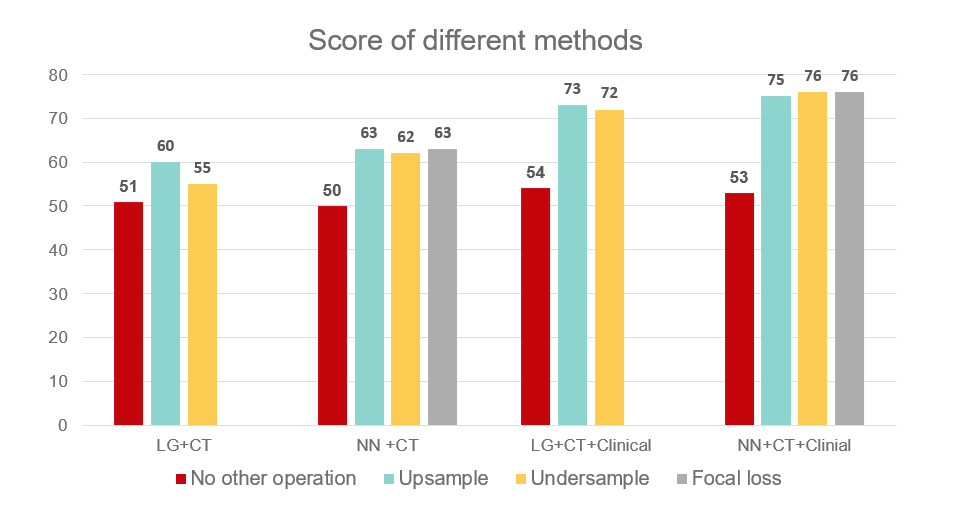
\includegraphics{plot/Balanced Score.png}
    \caption{Histogram on performances of various classification methods}
\end{center}
\end{figure}

By comparing the score in the above table, we make the following observations:

\begin{enumerate}
    \item All three strategies (Oversampling, Undersampling and Focal Loss) have significantly alleviated the negative impact of data imbalance. 
    \item The inclusion of clinical data that complements CT data improves the prediction of death outcome significantly across all methods.
    \item Neural Network shows a slightly better performance than Logistic Regression. 
\end{enumerate}

\subsection{Biological Age Prediction}

The next \textit{regression} task on biological age prediction is another type of prediction task that deviates from the classification in previous sections. As for the estimation of biological age, we make the assumption that patients with similar CT data should also have same implied biological ages, as they are more likely to share similar body characteristics. In particular, we choose to use \textbf{Linear Regression} and \textbf{Neural Network} to combine various features in CT data, and infer the biological ages from them. Also, we evaluate the performances by computing the residual loss for both linear regression and neural network.

\begin{figure}[h]
\centering     %%% not \center
\subfigure[Linear Regression, loss= 255]{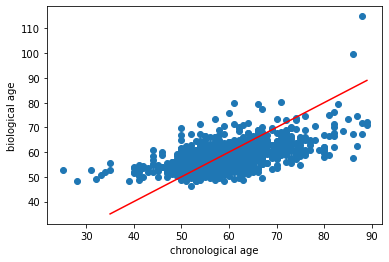
\includegraphics[width=80mm]{plot/Age_LR.png}}
\subfigure[Neural Network, loss= 250]{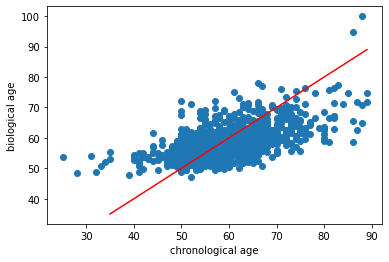
\includegraphics[width=80mm]{plot/Age_NN.png}}
\caption{Biological Age Regression}
\end{figure}

Figure 2 shows the results we obtain from the regression task. The red lines indicate the cases where chronological age coincides with the biological age. As a result, the performance of Linear Regression and Neural Network are similar. Both approaches ``shrink" the chronological ages to fit into middle ages, which means younger population tends to have higher biological age, and older population is more likely to have lower biological age. 

\section{Conclusion and Future Work}
In this project, we demonstrate that unused CT and clinical data contain insightful information in the prediction of adverse clinical outcomes as well as the inference of biological age of a patient. By introducing strategies to treat the highly imbalanced data set, utilizing logistic regression and neural network in supervised learning to perform the classification task, and using linear regression to conduct statistical inference, we have demonstrated that a number of features in the CT and clinical data have considerable potential to be integrated into routine clinical practices. 

In the future, one promising direction is to obtain substantial data on various types of clinical outcomes and conduct an improved \textit{multinomial} logistic regression. In this case, ML techniques could further support physicians with a more specified and accurate diagnosis. Also, as more clinical data becomes available, we would be able to test our algorithms on these new data and compare with other ML methods in a more systematic way. Finally, as for the regression task on biological age prediction, \textit{kNN regression} could provide alternative insights into the composition of similar groups of patients, which could also lead to more accurate and efficient clinical practices. We look forward to reviewing all possibilities to extend our current work.

\bibliographystyle{apalike}
\bibliography{biblio}

\end{document} 
































